\documentclass[fleqn]{article}
\oddsidemargin 0.0in
\textwidth 6.0in
\thispagestyle{empty}
\usepackage{import}
\usepackage{amsmath}
\usepackage{graphicx}
\usepackage[english]{babel}
\usepackage[utf8x]{inputenc}
\usepackage{float}
\usepackage{bigints} 
\usepackage[colorinlistoftodos]{todonotes}
\usepackage{setspace}
\usepackage{geometry}
\usepackage{colortbl}
\usepackage{xcolor,colortbl}

\definecolor{hwColor}{HTML}{AD53BA}

\doublespacing
\begin{document}

\begin{titlepage}

\newcommand{\HRule}{\rule{\linewidth}{0.5mm}} % Defines a new command for the horizontal lines, change thickness here

\center % Center everything on the page
 

\textsc{\LARGE Arizona State University}\\[1.5cm] 

\textsc{\LARGE Mathematical Methods For Physics I }\\[1.5cm]


\begin{figure}
  
\includegraphics[width=\linewidth]{asu.png}
\end{figure}


\HRule \\[0.4cm]
{ \huge \bfseries Portfolio}\\[0.4cm] 
\HRule \\[1.5cm]
 
\textbf{Behnam Amiri}

\bigbreak

\textbf{Prof: Cecilia Lunardini (Grader. Kenna McRae)}

\bigbreak


\textbf{{\large \today}\\[2cm]}

\vfill % Fill the rest of the page with whitespace

\end{titlepage}

\huge \textbf{Academic integrity statement:}

\bigbreak

\Large I am aware of the course rules detailed in the syllabus and related course documents. I am also aware of Arizona State University’s policies and practices against plagiarism and other forms of academic dishonesty. I affirm that I have not given or received any unauthorized help on this assignment, and I have not used any unauthorized resources. All authorized help (from the instructor, or learning assistant), authorized collaborations (with classmates), and authorized resources are explicitly stated and described in detail in the present document.

\bigbreak

\Large This work is entirely my own, except when collaboration with classmates is explicitly declared, and I take full responsibility for it.

\bigbreak

\Large Signature and date:

\bigbreak

\bigbreak



\includegraphics[height=3cm, width=6cm]{signature.jpg}

\Large \textbf{ Behnam Amiri, Novermber 2nd, 2020 }


\pagebreak

%  Table of contents
\begin{singlespace}
  \begin{tabular}{ |p{3cm}|||p{4cm}|p{2cm}|p{2cm}|p{2cm}|  }
      \hline
      Topic & Assignment & Page & Point Value & Points Earned \\
      \hline
      Complex numbers & \cellcolor{orange} Problems/Other & \cellcolor{orange} 3 &\cellcolor{orange}  ... &\cellcolor{orange}  ... \\
      & \cellcolor{orange} Exercises &\cellcolor{orange}  8 &\cellcolor{orange}  ... &\cellcolor{orange}  ... \\
      \hline
      Vectors & Problems/Other & 11 & ... & ... \\
      & Exercises & 13 & ... & ... \\
      \hline
      Matrcies & \cellcolor{orange} Problems/Other &\cellcolor{orange}  ... &\cellcolor{orange}  ... & \cellcolor{orange} ... \\
      & \cellcolor{orange} Exercises &\cellcolor{orange}  16 &\cellcolor{orange}  ... &\cellcolor{orange}  ... \\
      \hline
      Fourier Series & Problems/Other & ... & ... & ... \\
      & Exercises & ... & ... & ... \\
      \hline
      First-order Ordinary Diff. eg.  &\cellcolor{orange} Problems/Other &\cellcolor{orange} ... &\cellcolor{orange} ... &\cellcolor{orange} ... \\
      & \cellcolor{orange} Exercises &\cellcolor{orange}  ... &\cellcolor{orange}  ... &\cellcolor{orange}  ... \\
      \hline
      Second-order Ordinary Diff. eg. & Problems/Other & ...  & ... & ... \\
      & Exercises & ... & ... & ... \\
      \hline
      Other Ordinary Diff. eg. and important Diff eg. &\cellcolor{orange} Problems/Other &\cellcolor{orange} ... & \cellcolor{orange}... & \cellcolor{orange}...  \\ 
      & \cellcolor{orange} Exercises &\cellcolor{orange}  ... &\cellcolor{orange}  ... &\cellcolor{orange}  ... \\ 
      \hline
      Total & ... & ... & ... & ... \\
      \hline
  \end{tabular}
\end{singlespace}

\pagebreak

\vfill

\emph{ Important reminder: to get full credit, all calculations must be done by hand, without using electronic devices. Steps must be reasonably detailed.  The use of electronic devices is allowed, but must be explicitly declared, and will result in partial credit. See syllabus for details. Also see syllabus for rules on collaborating with others on a problem. } 

\bigbreak
\bigbreak

% Complex number start 

\textbf{Problem set on Complex Numbers} (40 points)

\begin{enumerate}

  \item  Solve the equation  $z^7-4z^6+6z^5-6z^4+6z^3-12z^2+8z+4=0,$

    \begin{enumerate}
      \item By examining the effect of setting $z^3$ equal to $2,$ and then 
      \item By factorising and using the binomial expansion of $(z+a)^4$

      \bigbreak

      Plot the seven roots of the equation on an Argand plot, exemplifying that complex roots of a polynomial equation always occur in conjugate pairs if the polynomial has real coefficients
    \end{enumerate}

  
  (Note: because the results are given at the end of the chapter, most of the  credit will be given for steps. ) 
  
  [Hint:  show that it is possible to factorize the equation as follows: $(z^3-2)(a z^4 + b z^3 + c z^2 + d z + e)=0$, with $a,b,c,d,e$ to be found. ]
  
  \item  Use de Moivre’s theorem with $n=4$ to prove that

  $cos(4\theta)=8cos^4(\theta)-8cos^2(\theta)+1$

  and deduce that 

  $cos(\dfrac{\pi}{8})=(\dfrac{2+\sqrt{2}}{4})^{1/2}$.

  \bigbreak

  \bigbreak


    \textcolor{hwColor}{
      $[cos(\theta)+isin(\theta)]^4=cos(4\theta)+isin(4\theta)$ \\
      \emph{L.H.S:} \\ 
      $[cos(\theta)+isin(\theta)]^4=[cos(\theta)+isin(\theta)]^2.[cos(\theta)+isin(\theta)]^2$ \\
      $=[cos^2(\theta)+i^2sin^2(\theta)+2icos(\theta)sin(\theta)].[cos^2(\theta)+i^2sin^2(\theta)+2icos(\theta)sin(\theta)]$ \\
      $=(cos^2(\theta)-sin^2(\theta)+2icos(\theta)sin(\theta)).(cos^2(\theta)-sin^2(\theta)+2icos(\theta)sin(\theta))$ \\
      $=cos^4(\theta)-cos^2(\theta)sin^2(\theta)+2icos^3(\theta)sin(\theta)-sin^2(\theta)cos^2(\theta)+sin^4(\theta)-2icos(\theta)sin^3(\theta)+2icos^3(\theta)sin(\theta)-2icos(\theta)sin^3(\theta)-4cos^2(\theta)sin^2(\theta)$ \\
      $=cos^4(\theta)+sin^4(\theta)-6cos^2(\theta)sin^2(\theta)+4icos^3(\theta)sin(\theta)-4icos(\theta)sin^3(\theta)$ \\
      $\Longrightarrow$ \emph{L.H.S:} \\
      $cos^4(\theta)+sin^4(\theta)-6cos^2(\theta)sin^2(\theta)+i[4cos^3(\theta)sin(\theta)-4cos(\theta)sin^3(\theta)]$ 
    }

    \textcolor{hwColor}{
      \emph{L.H.S = R.H.S} \\
      $cos^4(\theta)+sin^4(\theta)-6cos^2(\theta)sin^2(\theta)+i[4cos^3(\theta)sin(\theta)-4cos(\theta)sin^3(\theta)]=cos(4\theta)+isin(4\theta)$ \\
      $\longrightarrow$ $cos(4\theta)=cos^4(\theta)-6cos^2(\theta)sin^2(\theta)+sin^4(\theta)$ \\
      $cos(4\theta)=cos^4(\theta)-6cos^2(\theta)[1-cos^2(\theta)]+[1-cos^2(\theta)]^2$ \\
      $cos(4\theta)=cos^4(\theta)-6cos^2(\theta)+6cos^4(\theta)+1-2cos^2(\theta)+cos^4(\theta)$ \\
      $cos(4\theta)=8cos^4(\theta)-8cos^2(\theta)+1$ \thinspace \thinspace \thinspace  $\boxed{}$ \\
    }

    \bigbreak

    \textcolor{hwColor}{
      $cos(\dfrac{\pi}{8})=cos(4\dfrac{\pi}{32})=8cos^4(\dfrac{\pi}{32})-8cos^2(\dfrac{\pi}{32})+1$ \\
      From trigonometry we know that $cos(\dfrac{\theta}{2})=\sqrt{\dfrac{1+cos(\theta)}{2}}$ \\
      $cos(\dfrac{\pi}{32})=cos(\dfrac{\dfrac{\pi}{16}}{2})$ and $cos(\dfrac{\pi}{16})=cos(\dfrac{\dfrac{\pi}{8}}{2})$ \\
      $cos(\dfrac{\pi}{8})=\sqrt{\dfrac{1+cos(\dfrac{\pi}{4})}{2}}=\dfrac{\sqrt{2+\sqrt{2}}}{2}$ \\
      $cos(\dfrac{\pi}{16})=cos(\dfrac{\dfrac{\pi}{8}}{2})=\sqrt{\dfrac{1+cos(\dfrac{\pi}{8})}{2}}=\dfrac{\sqrt{2+\sqrt{2+\sqrt{2}}}}{2}$ \\
      $cos(\dfrac{\pi}{32})=cos(\dfrac{\dfrac{\pi}{16}}{2})=\sqrt{\dfrac{1+cos(\dfrac{\pi}{16})}{2}}=\dfrac{\sqrt{2+\sqrt{2+\sqrt{2+\sqrt{2}}}}}{2}$ \\
    }

    \textcolor{hwColor}{
      Let $cos(\dfrac{\pi}{32})=K$ \\
      $8K^4-8K^2+1=(\dfrac{2+\sqrt{2}}{4})^{1/2}$ \\
      Since $cos(\dfrac{\pi}{8})=8K^4-8K^2+1$ $\Longrightarrow cos(\dfrac{\pi}{8})=(\dfrac{2+\sqrt{2}}{4})^{1/2}$  \\
    }

  
  \item  In the theory of special relativity, the relationship between the position and time coordinates of an event, as measured in two frames of reference that have parallel $x-$ axes, can be expressed in terms of hyperbolic functions. If the coordinates are $x$ and $t$ in one frame and $x^\prime$ and $t^\prime$ in the other, then the relationship take the form
  
  $x^\prime=x cosh(\phi)-ct sinh(\phi),$
  
  $ct^\prime=-xsinh(\phi)+ct cosh(\phi)$.

  Express $x$ and $ct$ in terms of $x^\prime, ct^\prime$ and $\phi$ and show that 

  $x^2-(ct)^2=(x^\prime)^2-(ct^\prime)^2$
  
  \item The principal value of the logarithmic function of a complex variable is defined to have its argument in the range $-\pi < arg z\leq \pi $. By writting $z=tan(w)$ in terms of exponentials show that

  $tan^{-1}(z)=\dfrac{1}{2i} \ln(\dfrac{1+iz}{1-iz})$.

  Use this result to evaluate

  $tan^{-1}(\dfrac{2\sqrt{3}-3i}{7})$.
  
\end{enumerate}

% End of "Problem set on Complex Numbers"

\pagebreak

\textbf{Exercises set on Complex Numbers} (5 points)

\begin{enumerate}

  \item  Perform  the following computations, reducing the result to
  standard $a+ib$ form for complex numbers: 
  \[
  \begin{array}{lll}
  13.\,\frac{\textstyle 1+i}{\textstyle 1-i} & 14.\,\frac{\textstyle 2+i}{\textstyle i-1} & 15.\,\frac{\textstyle 4+5i}{\textstyle 5-3i} \\ 
  16.\,\frac{\textstyle 2+i}{\textstyle 3+2i}+\left( \frac{\textstyle i+4}{\textstyle 5i}\right)^{\ast} & 17.\,\frac{\textstyle i}{\textstyle 1+i}-\frac{\textstyle 1+i}{\textstyle i} & 18.\,\frac{\textstyle 3+5i}{\textstyle 5+3i}+4
  \end{array}
  \]
  
    \textcolor{hwColor}{
      13. $\dfrac{1+i}{1-i}=(\dfrac{1+i}{1-i}).(\dfrac{1+i}{1+i})=\dfrac{1+2i+i^2}{1^2+1^2}=i$
    }

    \textcolor{hwColor}{
      14. $\dfrac{2+i}{i-1}=(\dfrac{2+i}{i-1}).(\dfrac{i+1}{i+1})=\dfrac{2i+2+i^2+i}{i^2-1}=-(\dfrac{1}{2}+i\dfrac{3}{2})$
    }
    
    \textcolor{hwColor}{
      15. $\dfrac{4+5i}{5-3i}=(\dfrac{4+5i}{5-3i}).(\dfrac{5+3i}{5+3i})=\dfrac{20+12i+25i+15i^2}{25-9i^2}=\dfrac{5}{34}+i\dfrac{37}{34}$
    }

    \textcolor{hwColor}{
      16. $\dfrac{2+i}{3+2i}+(\dfrac{i+4}{5i})^*=\dfrac{2+i}{3+2i}+\dfrac{4-i}{-5i}=\dfrac{-5i(2+i)+(4-i)(3+2i)}{-5i(3+2i)}$ \\
      $=\dfrac{19-5i}{10-15i}=(\dfrac{19-5i}{10-15i}).(\dfrac{10+15i}{10+15i})=\dfrac{190+285i-50i-75i^2}{10^2+(15)^2}$ \\
      $=\dfrac{265+235i}{325}=\dfrac{53}{65}+i\dfrac{47}{65}$ \\
    }

    \textcolor{hwColor}{
      17. $\dfrac{i}{1+i}-\dfrac{1+i}{i}=\dfrac{i^2-(1+i)^2}{(1+i)i}=\dfrac{i^2-(1+2i+i^2)}{i+i^2}=\dfrac{-1-2i}{-1+i}$ \\
      $=(\dfrac{-1-2i}{-1+i}).(\dfrac{-1-i}{-1-i})=\dfrac{1+i+2i+2i^2}{2}=\dfrac{-1+3i}{2}$ \\
      $=-\dfrac{1}{2}+i\dfrac{3}{2}$ \\
    }

    \textcolor{hwColor}{
      18. $\dfrac{3+5i}{5+3i}+4=\dfrac{3+5i+20+12i}{5+3i}=\dfrac{23+17i}{5+3i}$ \\
      $=(\dfrac{23+17i}{5+3i}).(\dfrac{5-3i}{5-3i})=\dfrac{115-69i+85i-51i^2}{5^2+3^2}$ \\
      $=\dfrac{166+16i}{25+9}=\dfrac{83}{17}+i\dfrac{8}{17}$ \\
    }
  
  \item Perform the following calculations using the Euler (polar) form for \underline{each of the complex numbers} involved (in other words: take each number and transform it into polar form. Then, execute the operation given.).
  \[
  \begin{array}{lll}
  1.\;\left( 1+i\right) \left( 1-i\right)  & 2.\;\frac{\textstyle 1+i}{\textstyle 1+i\sqrt{3}} & 3.\;i\left( 3+4i\right)  \\ 
  4.\;\frac{\textstyle 1-3i}{\textstyle i} & 5.\;\frac{\textstyle 1+i}{\textstyle \sqrt{2}}\cdot \left( 1+i\sqrt{3}\right)  & 6.\;\left( 1+i\right) ^{5}
  \end{array}
  \]
  
  \item Express the following quantities in Cartesian $\left(x+iy\right) $ form and Euler $\left( re^{i\theta}\right)$ form. Indicate where there are multiple values.
  
  \begin{enumerate}
    \item $\exp \left( 1+i\sqrt{3}\right)$
    
    \item $\cos \left( 1+i\right)$
    
    \item $\sin \left( 1+i\right)$
    
    \item $\ln (2i)$
    
    \item $\ln \left( 1-i\pi \right)$
    
    \item $\cosh \left( 1+i\pi \right)$
  \end{enumerate}
  
  \item Compute the following roots and rational powers. Be sure to find all the solutions and plot them on an Argand plane. 
  \[
  \begin{array}{lll}
  1.\;i^{1/2} & 2.\;\left( -i\right) ^{1/2} & 3.\;2^{1/3} \\ 
  4.\;2^{2/3} & 5.\;(1+i\sqrt{3})^{3/5} & 6.\;\left( 1-i\right) ^{-2/3}
  \end{array}
  \]
  \end{enumerate}

% End of "Exercises set on Complex Numbers"

\pagebreak

% Complex numbers end


% Vectors start 

\textbf{Problem set on Vectors} (40 points)

\begin{enumerate}
  \item  Consider a 3-dimensional euclidean space, and the lines $s$ and $r$ given by the equations: 
    $$
    s~: ~ \begin{cases}
    x = t - 2 \\
    y=t \\ 
    z=2t-1 \\
    \end{cases} \hskip 1truecm r~: ~ \begin{cases}
      x-2=0 \\
      z+y=0 \\
    \end{cases}
    $$
    \begin{enumerate}
    \item Discuss if the two lines are parallel, intersecting or neither. 


    \item Determine if there exist two points, one on $s$ (call it $S$) and one on $r$ (call it $R$), such that the line $l$ passing by them is parallel to the planes $\alpha$ and $\beta$ defined below: 
    $$
    \alpha ~~:~~ x - 3z + 2 = 0 ~;\\
    ~~\beta : 2x - y = 1.
    $$
    If the answer is affirmative, find the points $R$ and $S$  and the equation of the line $l$. 

    \item verify your result by checking if the line $l$  intersects the planes $\alpha$ and $\beta$.  Discuss as needed. 
    \end{enumerate}

  \item Consider the planes $\pi_1$, $\pi_2$ and $\pi_3$ described by the equations: 
    \begin{eqnarray}
    &&\pi_1 ~~ :~~ z-3=0 \nonumber \\
    &&\pi_2 ~~ :~~ x+y+2=0 \nonumber \\
    &&\pi_3 ~~ :~~ 3x+3y-z+9=0 ~.\nonumber 
    \end{eqnarray}
    Consider also the line $r$ given by the intersection of $\pi_1$ and $\pi_2$. 
    \begin{enumerate}

    \item establish if the plane $\pi_3$ contains $r$. 

    \item  find the equation of the plane $\pi_4$ which passes by the origin and contains $r$. 

    \item find the point $O^\prime$ defined as the (orthogonal) projection of the origin on the plane $\pi_1$. 
  \end{enumerate}

  \item Consider the planes $\pi_1$, $\pi_2$ and $\pi_3$ described by the equations: 
    \begin{eqnarray}
    &&\pi_1 ~~ :~~ 2x-y=1 \nonumber \\
    &&\pi_2 ~~ :~~ x+y+z=0 \nonumber \\
    &&\pi_3 ~~ :~~ x-2z=1 ~.\nonumber 
    \end{eqnarray}
    \begin{enumerate}
    \item Find the point $A$ of intersection of the three planes. 

    \item  find the plane $\pi_4 $ that passes by the origin and is orthogonal to the line $r$, defined as the intersection of $\pi_1$ and $\pi_2$. 

    \item Calculate the area of the triangle with vertices $A$, $B$ and $C$, where $B$ is the intersection of  $\pi_1$, $\pi_3$ and $\pi_4$, and $C$ is the intersection of $\pi_2$, $\pi_3$ and $\pi_4$. 

    \end{enumerate}


  \item Define as $r$ the line passing by the points A = (0, 0, 1) and B = (-2, -1, 0). Likewise, let $s$ be the line passing by the points C = (1,1,1) and D = (-1,0,0).
    \begin{enumerate}
    \item prove that the two lines are coplanar and find the equation of the plane $\pi$ that contains them both. 

    \item find the parametric equation describing the line passing by the origin and orthogonal to $\pi$. 
    \end{enumerate}

\end{enumerate}

\pagebreak

\textbf{Exercises set on Vectors} (5 points)

\begin{enumerate}

  \item You are given the following vectors in terms of their components in
  the $\left\{ \mathbf{\hat{x}},\,\mathbf{\hat{y}},\mathbf{\, \hat{z}}\right\} $ basis: 
  \[
  \mathbf{A}=\mathbf{\hat{x}}+2\mathbf{\hat{y}-}2\mathbf{\hat{z}, \quad \quad B}=3\mathbf{\hat{x}}+\mathbf{\hat{y}+}2\mathbf{\hat{z}, \quad \quad C}=4\mathbf{\hat{x}}-\mathbf{\hat{y}+\hat{z}.}
  \]
  Take $\theta_{\rm AC}$ to be the angle between vectors $\mathbf{A}$ and $\mathbf{C}$, etc. 
  
  \begin{enumerate}
    \item Prove that these vectors are linearly independent. 
    
    \item Compute  $\mathbf{A\times B,\;A\times C}$ and $\mathbf{B\times C}$
    
    \item Compute (by hand) $\cos \theta_{\rm AB},\,\cos \theta_{\rm AC},\,\cos \theta_{\rm BC}$
    
    \item Compute (by hand) $\sin \theta_{\rm AB},\,\sin \theta_{\rm AC},\,\sin \theta_{\rm BC}$
    
    \item Compute $\mathbf{A\cdot }\left( \mathbf{B\times C}\right) ,\;\mathbf{B\cdot }\left( \mathbf{A\times C}\right) $ and $\mathbf{C\cdot }\left( \mathbf{A\times B}\right)$
    
    \item Compute $\left( \mathbf{A\times B}\right) \times \mathbf{C+}\left( \mathbf{B\times C}\right) \times \mathbf{A+}\left( \mathbf{C\times A}\right) \times \mathbf{B}$
  \end{enumerate}
  
  
  \item Find an equation of the plane through the points $\left(
  0,\,0,\,3\right) ,\;\left( 1,\,1,\,1\right) $ and $\left( -1,\,1,\,2\right) $.
  
  \item Find the equation of the plane that contains the point $\left(
  2,\,1,\,-4\right) $ and is perpendicular to the vector $3\mathbf{\hat{x}}-2\mathbf{\hat{y}}+\mathbf{\hat{z}}.$
  
  \item Determine $b$ such that the line through $\left( 5,\,0,\,3\right) $ and $\left( -1,\,-10,\,b\right) $ will be perpendicular to $\left( \mathbf{\hat{x}+\hat{y}}\right) \mathbf{\times }\left( \mathbf{\hat{x}+\hat{z}}\right)$.
  
  \item Use vectors to find the equation of the straight line containing the points $\left( 1,\,-2,\,4\right) $ and $\left( 6,\,1,\,1\right) .$ Write this equation in \emph{parametric form}, {\it i.e.}, in the form $\mathbf{r}= \mathbf{r}_{0}+t\mathbf{V}$, where $\mathbf{r}_{0}$ is the vector describing a given point on the line, $\mathbf{V}$ is a vector oriented along the line, and $t$ is a variable that has range $\left( -\infty ,\,\infty \right)$. 
  
  \item Find the vector(s) having modulus equal to $\sqrt{13}$, which are orthogonal to the $y$-axis and parallel to the plane $3x - 2z -5=0$.
  
  \item Considerate the lines $r$ and $s$, given by the  equations: 
  \begin{equation}
  r: 
  \begin{cases} x-2= 0 \\ z+y=0    \end{cases} ; ~~~~~~   s: \begin{cases} x = t - 2  \\ y=t \\ 2t- 1   \end{cases}   
  \end{equation}
  %\end{equation}
  Establish if it is possible to find a point $R$ located on $r$, and a point $S$ located on $s$, so that the line passing by $R$ and $S$ 
  is parallel to the planes 
  $\alpha : x - 3z + 2 = 0$ and  $\beta : 2x - y = 1$.
  
  \item 
  %Fis, i, j, k, determinare equazioni parametriche della retta passante per P = (1, 3, 0), parallela al piano yz e al piano $x + y + z = 0$.
  
  Find a parametric equation describing the line passing by the point $P = (1, 3, 0)$, and parallel to both the $x=0$ plane (i.e., the $yz$ plane) and the plane $x + y + z = 0$. 
  
  \end{enumerate}
% End of "Exercises set on Vectors"

\pagebreak

\textbf{Problem set on Matrices} (40 points)

\begin{enumerate}


  \item Consider the following vectors: $ \mathbf{A}=\left( 1,2,-1\right) \mathbf{,\;B}=\left( 1,2,2\right), \mathbf{C}=\left( 1,0,1\right)$.
  
    \begin{enumerate}
    \item Test to see if these three vectors are linearly independent.
  
    \item Construct, \textbf{using the Gram-Schmidt orthogonalization method}, three different sets of orthonormal three-dimensional basis vectors. In the first one, take one basis vector in the direction of $\mathbf{A}$, the second in the $\mathbf{A}$-$\mathbf{B}$ plane and the third perpendicular to that plane in a right-handed sense. In the second one, start with $\mathbf{B}$, take the second basis vector to be in the $\mathbf{B}$-$\mathbf{C}$ plane, etc. (There is an easier way than the Gram-Schmidt process to do these particular problems, but please use the Gram-Schmidt process in this exercise.)
    \end{enumerate}
  
  
  \item  Two of the following matrices are Hermitian. Pick them out and dismiss the rest; you will not need them again. 
    \[
    \left( a\right) \,\left( 
    \begin{array}{lll}
    0 & -i & 0 \\ 
    i & 0 & 0 \\ 
    0 & 0 & 0
    \end{array}
    \right) \;\left( b\right) \,\left( 
    \begin{array}{lll}
    0 & 0 & i \\ 
    0 & 0 & 0 \\ 
    i & 0 & 0
    \end{array}
    \right) \;\left( c\right) \,\left( 
    \begin{array}{lll}
    0 & 0 & 0 \\ 
    0 & 0 & 1 \\ 
    0 & -1 & 0
    \end{array}
    \right) \;\left( d\right) \,\left( 
    \begin{array}{lll}
    0 & 0 & 1 \\ 
    0 & 0 & 0 \\ 
    1 & 0 & 0
    \end{array}
    \right) 
    \]
  
  
    \begin{enumerate}
    \item  Find the eigenvalues and orthonormal sets of eigenvectors for each of the two Hermitian matrices. (Neither one is degenerate.)
  
    \item  If you have done the previous part correctly, you will have found
    that the two matrices have the same eigenvalues. Consequently, 
    by diagonalization, they correspond to the same diagonal matrix. Prove \emph{in general }that any two Hermitian matrices, $\mathsf{H}_{1}$ and $\mathsf{H}_{2}$ (of
    the same dimension), that correspond to the same diagonal matrix (i.e., have the same eigenvalues) are related to each other by a unitary transformation.
    That is to say, there exists a unitary matrix $\mathsf{U}$ such that $%
    \mathsf{H}_{1}=\mathsf{U}^{\dagger }\mathsf{H}_{2}\mathsf{U}$. Do this by
    showing what $\mathsf{U}$ should be. [Hint: How do you actually diagonalize
    a Hermitian matrix?]
  
    \item Illustrate this theorem explicitly, using the two Hermitian matrices you have
    ``diagonalized'' above as an example. 
  
    \end{enumerate}
  
  \item We have a matrix equation of the type $\mathsf{M}\,\mathsf{v}=\mathsf{b}$, given by
    \[
      \left(
      \begin{array}{rrrr}
          0 & 1 & 2 & 1 \\
          2 & 1 & 2 & 1 \\
          -1 & 3 & 3 & -1 \\
          3 & 1 & 2 & 2 \\
      \end{array}
      \right)
      \left(
      \begin{array}{c}
          x \\
          y \\
          z \\
          t \\
      \end{array}
      \right)
      =
      \left(
      \begin{array}{c}
          2 \\
          4 \\
          2 \\
          5  \\
      \end{array}
      \right).
    \]
    Find the determinant $\left| \mathsf{M} \right|$,  the inverse matrix $\mathsf{M}^{-1}$ (using any method of your choice), and solve for the vector $\mathsf{v}$.

      \textcolor{hwColor}{
        $
          det(M)= \\
          2(-1)^{2+1}
          \begin{vmatrix}
            1 & 2 & 1 \\ 
            3 & 3 & -1 \\
            1 & 2 & 2 \\
          \end{vmatrix}+
          (-1)(-1)^{3+1} 
          \begin{vmatrix}
            1 & 2 & 1 \\ 
            1 & 2 & 1 \\
            1 & 2 & 2 \\
          \end{vmatrix}+
          3(-1)^{4+1}
          \begin{vmatrix}
            1 & 2 & 1 \\ 
            1 & 2 & 1 \\
            3 & 3 & -1 \\
         \end{vmatrix}
        $
      }

      \textcolor{hwColor}{
        Assume 
        $
          A=\begin{vmatrix}
            1 & 2 & 1 \\ 
            3 & 3 & -1 \\
            1 & 2 & 2 \\
          \end{vmatrix} ~~~
          B=\begin{vmatrix}
            1 & 2 & 1 \\ 
            1 & 2 & 1 \\
            1 & 2 & 2 \\
          \end{vmatrix} ~~~
          C=\begin{vmatrix}
            1 & 2 & 1 \\ 
            1 & 2 & 1 \\
            3 & 3 & -1 \\
         \end{vmatrix}
        $
      }

      \bigbreak

      \textcolor{hwColor}{
        Then
        $det(M)=-(2A+B+3C)$
      }

      \bigbreak

      \textcolor{hwColor}{
        $
          det(A)=\begin{vmatrix}
            1 & 2 & 1 \\ 
            3 & 3 & -1 \\
            1 & 2 & 2 \\
          \end{vmatrix} \\
          =(-1)^{1+1}(6+2)+2(-1)^{1+2}(6+1)+(-1)^{1+3}(6-3)=8-14+3=-3
        $
      }

      \bigbreak

      \textcolor{hwColor}{
        $
        det(B)=\begin{vmatrix}
          1 & 2 & 1 \\ 
          1 & 2 & 1 \\
          1 & 2 & 2 \\
        \end{vmatrix} \\
        =(-1)^{1+1}(4-2)+2(-1)^{1+2}(2-1)+(-1)^{1+3}(2-2)=2-2+0=0
        $
      }

      \bigbreak

      \textcolor{hwColor}{
        $
        det(C)=\begin{vmatrix}
          1 & 2 & 1 \\ 
          1 & 2 & 1 \\
          3 & 3 & -1 \\
        \end{vmatrix} \\
        =(-1)^{1+1}(-2-3)+2(-1)^{1+2}(-1-3)+(-1)^{1+3}(3-6)=-5+8-3=0
        $
      }

      \bigbreak

      \textcolor{hwColor}{
        $
          det(M)=-\left[2A+B+3C\right]=-\left[2(-3)+0+0\right] \\
          \Longrightarrow det(M)=6
        $
      }

      \rule{16cm}{0.4pt}

      \textcolor{hwColor}{
        $
          M^{-1}= \dfrac{adj(M)}{det(M)}, ~~~
          M=\begin{pmatrix}
            0 & 1 & 2 & 1 \\
            2 & 1 & 2 & 1 \\
            -1 & 3 & 3 & -1 \\
            3 & 1 & 2 & 2 \\
          \end{pmatrix} \\
        $
      }

      \textcolor{hwColor}{ 
        $
          adj(M)=
            \begin{pmatrix}
              +det(M_{11}) & -det(M_{12}) & +det(M_{13}) & -det(M_{14}) \\ 
              -det(M_{21}) & +det(M_{22}) & -det(M_{23}) & +det(M_{24}) \\ 
              +det(M_{31}) & -det(M_{32}) & +det(M_{33}) & -det(M_{34}) \\ 
              -det(M_{41}) & +det(M_{42}) & -det(M_{43}) & +det(M_{44}) 
            \end{pmatrix}^T \\
          M_{11}=
            \begin{pmatrix}
              1 & 2 & 1 \\ 
              3 & 3 & -1 \\ 
              1 & 2 & 2
            \end{pmatrix},
          M_{12}=
            \begin{pmatrix}
            2 & 2 & 1 \\ 
            -1 & 3 & -1 \\ 
            3 & 2 & 2
            \end{pmatrix},
          M_{13}=\begin{pmatrix}
            2 & 1 & 1 \\ 
            -1 & 3 & -1 \\ 
            3 & 1 & 2
            \end{pmatrix} \\
          M_{14}=
            \begin{pmatrix}
            2 & 1 & 2 \\ 
            -1 & 3 & 3 \\ 
            3 & 1 & 2
            \end{pmatrix},
          M_{21}=
            \begin{pmatrix}
            1 & 2 & 1 \\ 
            3 & 3 & -1 \\ 
            1 & 2 & 2
            \end{pmatrix},
          M_{22}=\begin{pmatrix}
            0 & 2 & 1 \\ 
            -1 & 3 & -1 \\ 
              3 & 2 & 2
            \end{pmatrix} \\
          M_{23}=
            \begin{pmatrix}
            0 & 1 & 1 \\ 
            -1 & 3 & -1 \\ 
              3 & 1 & 2
            \end{pmatrix},
          M_{24}=
            \begin{pmatrix}
            0 & 1 & 2 \\ 
            -1 & 3 & 3 \\ 
            3 & 1 & 2
            \end{pmatrix},
          M_{31}=\begin{pmatrix}
            1 & 2 & 1 \\ 
            1 & 2 & 1 \\ 
            1 & 2 & 2
            \end{pmatrix} \\
          M_{32}=
            \begin{pmatrix}
            0 & 2 & 1 \\ 
            2 & 2 & 1 \\ 
            3 & 2 & 2
            \end{pmatrix},
          M_{33}=
            \begin{pmatrix}
            0 & 1 & 1 \\ 
            2 & 1 & 1 \\ 
            3 & 1 & 2
            \end{pmatrix},
          M_{34}=\begin{pmatrix}
            0 & 1 & 2 \\ 
            2 & 1 & 2 \\ 
            3 & 1 & 2
            \end{pmatrix} \\
          M_{41}=
            \begin{pmatrix}
            1 & 2 & 1 \\ 
            1 & 2 & 1 \\ 
            3 & 3 & -1
            \end{pmatrix},
          M_{42}=
            \begin{pmatrix}
            0 & 2 & 1 \\ 
            2 & 2 & 1 \\ 
            -1 & 3 & -1
            \end{pmatrix},
          M_{43}=\begin{pmatrix}
            0 & 1 & 1 \\ 
            2 & 1 & 1 \\ 
            -1 & 3 & -1
            \end{pmatrix} \\
          M_{44}=
            \begin{pmatrix}
            0 & 1 & 2 \\
            2 & 1 & 2 \\
            -1 & 3 & 3 
            \end{pmatrix} \\
          adj(M)=
            \begin{pmatrix}
            -3 & 3 & 0 & 0  \\ 
            -3 & -13 & 4 & 10 \\ 
            3 & 11 & -2 & -8  \\ 
            3 & -9 & 0 & 6 
            \end{pmatrix} \\
          M^{-1}=\dfrac{adj(M)}{det(M)}=\dfrac{ \begin{pmatrix}
            -3 & 3 & 0 & 0  \\ 
            -3 & -13 & 4 & 10 \\ 
            3 & 11 & -2 & -8  \\ 
            3 & -9 & 0 & 6 
          \end{pmatrix}}{6} \\
          \\
          \Longrightarrow M^{-1}=\begin{pmatrix}
            -\dfrac{1}{2} & \dfrac{1}{2} & 0 & 0 \\
            \\
            -\dfrac{1}{2} & -\dfrac{13}{6} & \dfrac{2}{3} & \dfrac{5}{3} \\
            \\
            \dfrac{1}{2} & \dfrac{11}{6} & -\dfrac{1}{3} & -\dfrac{4}{3} \\
            \\ 
            \dfrac{1}{2} & -\dfrac{3}{2} & 0 & 1 \\ 
          \end{pmatrix}
        $
      }

      \textcolor{hwColor}{
        $
          Mv=b \\
          M^{-1}Mv=M^{-1}b \\
          Iv=M^{-1}b \\
          \rightarrow v=M^{-1}b\\
          =\begin{pmatrix}
            -\dfrac{1}{2} & \dfrac{1}{2} & 0 & 0 \\
            \\
            -\dfrac{1}{2} & -\dfrac{13}{6} & \dfrac{2}{3} & \dfrac{5}{3} \\
            \\
            \dfrac{1}{2} & \dfrac{11}{6} & -\dfrac{1}{3} & -\dfrac{4}{3} \\
            \\ 
            \dfrac{1}{2} & -\dfrac{3}{2} & 0 & 1 \\ 
          \end{pmatrix}.\begin{pmatrix}
            2 \\
            4 \\
            2 \\
            5 \\
          \end{pmatrix}
        $
      }

      \textcolor{hwColor}{
        $
          =\begin{pmatrix}
            -\dfrac{2}{2}+\dfrac{4}{2}+0+0 \\
            -\dfrac{2}{2}+\dfrac{-13}{6}4+\dfrac{4}{3}+\dfrac{25}{3} \\
            \dfrac{2}{2}+\dfrac{44}{6}+\dfrac{-2}{3}+\dfrac{-20}{3} \\
            \dfrac{2}{2}+\dfrac{-12}{2}+0+5 \\
          \end{pmatrix}
          \Longrightarrow \begin{pmatrix}
            x \\
            y \\
            z \\
            t \\
          \end{pmatrix}=\begin{pmatrix}
            1 \\
            0 \\
            1 \\
            0 \\
          \end{pmatrix}
        $
      }



    If the column matrix $\mathsf{b}$ on the right is changed to 
    \[
      \mathsf{b}
      =
      \left(
      \begin{array}{c}
          1 \\
          1 \\
          1 \\
          1 \\
      \end{array}
      \right),
    \]
    and $\mathsf{M}$ is unchanged, what is the new solution $\mathsf{v}$?
  
  
  \item Consider the matrix:
    $$
    A=\left(
    \begin{array}{ccc}
    1 & 1 & h \\
    2 & h & 2 \\
    3 & h & 3 \\
    \end{array}
    \right)~,
    $$
    where $h$ is a real parameter.  
    \begin{itemize}
    \item Find the rank of A for varying values of $h$ (i.e., discuss all possible distinct cases depending on the value of $h$.) 
  
    \item  For $h=0$, find the eigenvalues and the eigenvectors of $A$, and construct the matrix $U$ that diagonalizes $A$. 
  
    \item Attempt to repeat the step above for $h=1$: obtain the eigenvalues and discuss how in this case the matrix can not be diagonalized. Discuss as adequate. 
    \end{itemize}
  
  
  \end{enumerate}

\pagebreak


\textbf{Exercises set on Matrices} (5 points)

\begin{enumerate}

  \item Determine which of the following matrices have inverses by computing their determinants (5 point per determinant).
    \begin{eqnarray*}
      &&\rm{(A) }\left( 
      \begin{array}{rrr}
      3 & 1 & 5 \\ 
      -1 & -3 & -1 \\ 
      2 & 2 & 3
      \end{array}
      \right) ;\;\rm{(B) }\left( 
      \begin{array}{rrr}
      6 & -2 & 3 \\ 
      1 & 1 & 1 \\ 
      2 & -3 & 1
      \end{array}
      \right) ;\;\rm{(C) }\left( 
      \begin{array}{rrr}
      4 & 2 & 2 \\ 
      -1 & 3 & -1 \\ 
      3 & 4 & 5
      \end{array}
      \right) ;\; \\
      &&\rm{(D)\ }\left( 
      \begin{array}{rrrr}
      2 & 3 & -1 & 1 \\ 
      3 & -4 & 3 & -1 \\ 
      2 & -1 & 1 & -3 \\ 
      3 & 1 & -2 & 4
      \end{array}
      \right) ;\;
    \end{eqnarray*}

    % Answer 

    \textcolor{hwColor}{
      $
        det(A)=
        3(-1)^{1+1}
        \begin{pmatrix}
          -3 & -1 \\ 
          2 & 3
        \end{pmatrix}
        +
        1(-1)^{1+2}
        \begin{pmatrix}
          -1 & -1 \\ 
          2 & 3
        \end{pmatrix}
        +
        5(-1)^{1+3}
        \begin{pmatrix}
          -1 & -3 \\ 
          2 & 2
        \end{pmatrix} \\
        = 3(-9-(-2))+(-1)(-3-(-2)+5(-2-(-6)) \\
        \Longrightarrow det(A)=0 \\
        \emph{Matrix A is singular therefore it is NOT invertible.}
      $
    }

    \rule{16cm}{0.4pt}

    \textcolor{hwColor}{
      $
        det(B)=
        (6)(-1)^{1+1}
        \begin{pmatrix}
          1 & 1 \\ 
          -3 & 1
        \end{pmatrix}
        +
        (-2)(-1)^{1+2}
        \begin{pmatrix}
          1 & 1 \\ 
          2 & 1
        \end{pmatrix}
        +
        (3)(-1)^{1+3}
        \begin{pmatrix}
          1 & 1 \\ 
          2 & -3
        \end{pmatrix} \\
        = 6(1-(-3))+(2)(1-2)+(3)(-3-2) \\
        \Longrightarrow det(B)=7 \\
        \emph{Matrix B is invertible.}
      $
    }

    \rule{16cm}{0.4pt}

    \textcolor{hwColor}{
      $
        det(C)=
          (4)(-1)^{1+1}
          \begin{pmatrix}
            3 & -1 \\ 
            4 & 5
          \end{pmatrix}
          +
          (2)(-1)^{1+2}
          \begin{pmatrix}
            -1 & -1 \\ 
            3 & 5
          \end{pmatrix}
          +
          (2)(-1)^{1+3}
          \begin{pmatrix}
            -1 & 3 \\ 
            3 & 4
          \end{pmatrix} \\
        = 4(15-(-4))+(-2)(-5-(-3))+(2)(-4-9) \\
        \Longrightarrow det(C)= 54 \\
        \emph{Matrix C is invertible.}
      $
    }

    \rule{16cm}{0.4pt}

    \textcolor{hwColor}{
      $
      det(D)=
        (2)(-1)^{1+1}
        \begin{pmatrix}
          -4 & 3 & -1 \\ 
          -1 & 1 & -3 \\ 
          1 & -2 & 4
        \end{pmatrix}
        +
        (3)(-1)^{2+1}
        \begin{pmatrix}
          3 & -1 & 1 \\ 
          -1 & 1 & -3 \\ 
          1 & -2 & 4
        \end{pmatrix}
        +
        (2)(-1)^{3+1}
        \begin{pmatrix}
         3 & -1 & 1 \\ 
         -4 & 3 & -1 \\ 
         1 & -2 & 4
        \end{pmatrix}
        +
        (3)(-1)^{4+1}
        \begin{pmatrix}
         3 & -1 & 1 \\ 
         -4 & 3 & -1 \\ 
         -1 & 1 & -3
        \end{pmatrix} \\
        = 2[-4(4-6)-3(-4+3)-(2-1)]+(-3)[3(4-6)+(-4+3)+(2-1)]
        + 2[3(12-2)+(-16+1)+(8-3)]+(-3)[3(-9+1)+(12-1)+(-4+3)] \\
      = 20+18+40+42 \\
      \Longrightarrow det(D)= 120 \\
      \emph{Matrix D is invertible.} \\
      $
    }


  \item Continue the previous exercise: for the matrices that have non-vanishing determinants, compute the inverses using a method of your choice (5 points for each inverse calculation). 
    \textcolor{hwColor}{ \\
      \emph{The adjoint of a matrix is the transpose of the cofactor matrix of that matrix.} \\
        $
          B=\begin{pmatrix}
            6 & -2 & 3 \\ 
            1 & 1 & 1 \\ 
            2 & -3 & 1
          \end{pmatrix}
          ,
          adj(B)=
          \begin{pmatrix}
          4 & 1 & -5 \\
          -7 & 0 & 14 \\
          -5 & -3 & 8
          \end{pmatrix}^T \\
          ,
          det(B)=7, ~~~B^{-1}= \dfrac{adj(B)}{det(B)}=\dfrac{
          \begin{pmatrix}
            4 & -7 & -5 \\
            1 & 0 & -3 \\
            -5 & 14 & 8
          \end{pmatrix}
        }{7}=
        \begin{pmatrix}
          \dfrac{4}{7} & -1 & \dfrac{-5}{7} \\
          \dfrac{1}{7} & 0 & \dfrac{-3}{7} \\
          \dfrac{-5}{7} & 2 & \dfrac{8}{7}
        \end{pmatrix}
      $
    }

    \rule{16cm}{0.4pt}

    \textcolor{hwColor}{
      $
        C=\begin{pmatrix}
          4 & 2 & 2 \\ 
          -1 & 3 & -1 \\ 
          3 & 4 & 5
        \end{pmatrix}
        ,
        adj(C)=
        \begin{pmatrix}
        19 & 2 & -13 \\
        -2 & 14 & -10 \\
        -8 & 2 & 14
        \end{pmatrix}^T
        ,
        det(C)=54 \\
      C^{-1}= \dfrac{adj(C)}{det(C)}=\dfrac{
        \begin{pmatrix}
          19 & -2 & -8 \\
          2 & 14 & 2 \\
          -13 & -10 & 14
        \end{pmatrix}
      }{54}
      =
      \begin{pmatrix}
        \dfrac{19}{54} & \dfrac{-1}{27} & \dfrac{-4}{27} \\
        \dfrac{1}{27} & \dfrac{7}{27} & \dfrac{1}{27} \\
        \dfrac{-13}{54} & \dfrac{-5}{27} & \dfrac{7}{27}
      \end{pmatrix}
      $
    }

    \rule{16cm}{0.4pt}

    \textcolor{hwColor}{ 
      $
        D=
        \begin{pmatrix}
          2 & 3 & -1 & 1 \\ 
          3 & -4 & 3 & -1 \\ 
          2 & -1 & 1 & -3 \\ 
          3 & 1 & -2 & 4
        \end{pmatrix} \\
        adj(D)=
          \begin{pmatrix}
            +det(D_{11}) & -det(D_{12}) & +det(D_{13}) & -det(D_{14}) \\ 
            -det(D_{21}) & +det(D_{22}) & -det(D_{23}) & +det(D_{24}) \\ 
            +det(D_{31}) & -det(D_{32}) & +det(D_{33}) & -det(D_{34}) \\ 
            -det(D_{41}) & +det(D_{42}) & -det(D_{43}) & +det(D_{44}) 
          \end{pmatrix}^T \\
        D_{11}=
          \begin{pmatrix}
            -4 & 3 & -1 \\ 
            -1 & 1 & -3 \\ 
            1 & -2 &  4
          \end{pmatrix},
          D_{12}=
          \begin{pmatrix}
          3 & 3 & -1 \\
          2 & 1 & -3 \\
          3 & -2 & 4 
          \end{pmatrix},
          D_{13}=\begin{pmatrix}
          3 & -4 & -1 \\
          2 & -1 & -3 \\
          3 & 1 &  4 
          \end{pmatrix} \\
        D_{14}=
          \begin{pmatrix}
          3 & -4 & 3 \\
          2 & -1 & 1 \\
          3 & 1 &  -2
          \end{pmatrix},
          D_{21}=
          \begin{pmatrix}
          3 & -1 & 1 \\
          -1 & 1 & -3 \\
          1 & -2 &  4
          \end{pmatrix},
          D_{22}=\begin{pmatrix}
          2 & -1 & 1 \\
          2 & 1 & -3 \\
          3 & -2 & 4 
          \end{pmatrix} \\
        D_{23}=
          \begin{pmatrix}
          2 & 3 & 1 \\
          2 & -1 & -3 \\
          3 & 1 & 4 
          \end{pmatrix},
          D_{24}=
          \begin{pmatrix}
          2 & 3 & -1 \\
          2 & -1 & 1 \\
          3 & 1 & -2 
          \end{pmatrix},
          D_{31}=\begin{pmatrix}
          3 & -1 & 1 \\
          -4 & 3 & -1 \\
          1 & -2 & 4 
          \end{pmatrix} \\
        D_{32}=
          \begin{pmatrix}
          2 & -1 & 1 \\
          3 & 3 & -1 \\
          3 & -2 & 4 
          \end{pmatrix},
          D_{33}=
          \begin{pmatrix}
          2 & 3 & 1 \\
          3 & -4 & -1 \\
          3 & 1 & 4 
          \end{pmatrix},
          D_{34}=\begin{pmatrix}
          2 & 3 & -1 \\
          3 & -4 & 3 \\
          3 & 1 & -2 
          \end{pmatrix} \\
        D_{41}=
          \begin{pmatrix}
          3 & -1 & 1 \\
          -4 & 3 & -1 \\
          -1 & 1 & -3 
          \end{pmatrix},
          D_{42}=
          \begin{pmatrix}
          2 & -1 & 1 \\
          3 & 3 & -1 \\
          2 & 1 & -3 
          \end{pmatrix},
          D_{43}=\begin{pmatrix}
          2 & 3 & 1 \\
          3 & -4 & -1 \\
          2 & -1 & -3
          \end{pmatrix} \\
        D_{44}=
          \begin{pmatrix}
          2 & 3 & -1 \\
          3 & -4 & 3 \\
          2 & -1 & 1 
          \end{pmatrix} \\
        adj(D)=
          \begin{pmatrix}
          10 & 6 & 20 & 14 \\ 
          50 & 6 & -20 & -26 \\ 
          60 & 48 & -60 & -48 \\ 
          10 & 18 & -40 & 2
          \end{pmatrix} \\
        D^{-1}= \dfrac{adj(D)}{det(D)}=\dfrac{
          \begin{pmatrix}
            \dfrac{10}{120} & \dfrac{6}{120} & \dfrac{20}{120} & \dfrac{14}{120} \\ 
            \dfrac{50}{120} & \dfrac{6}{120} & \dfrac{-20}{120} & \dfrac{-26}{120} \\ 
            \dfrac{60}{120} & \dfrac{48}{120} & \dfrac{-60}{120} & \dfrac{-48}{120} \\ 
            \dfrac{10}{120} & \dfrac{18}{120} & \dfrac{-40}{120} & \dfrac{2}{120}
          \end{pmatrix}
        }{120}=
        \begin{pmatrix}
          \dfrac{1}{12} & \dfrac{1}{20} & \dfrac{1}{6} & \dfrac{7}{60} \\ 
          \dfrac{5}{12} & \dfrac{1}{20} & \dfrac{-1}{6} & \dfrac{-13}{60} \\ 
          \dfrac{1}{2} & \dfrac{2}{5} & \dfrac{-1}{2} & \dfrac{-2}{5} \\  
          \dfrac{1}{12} & \dfrac{3}{20} & \dfrac{-1}{3} & \dfrac{1}{60}
        \end{pmatrix}
      $
    }

  
  \item  Consider the following vectors (column matrices):
    \[
    \mathsf{A}=\left( 
    \begin{array}{l}
    2 \\ 
    3
    \end{array}
    \right) ,\;\mathsf{B}=\left( 
    \begin{array}{l}
    1 \\ 
    5
    \end{array}
    \right) ,
    \]

  Rotate ({\it i.e.}, find the necessary rotation matrix) $\mathsf{A}$ into the direction of $\mathsf{B}$.


  \item  For each of the following matrices, (a) compute the trace, (b) write down the Hermitian adjoint, and (c) determine whether it is Hermitian, unitary or neither. \emph{( answering all the questions for each matrix is worth 5 points. Be careful and try to answer the questions in the most efficient way, avoiding unnecessary calculations)}. 
    \[
    \begin{array}{ccccc}
    1. & A=\left( 
    \begin{array}{ccc}
    1 & 0 & -i \\ 
    0 & -2 & 4-i \\ 
    i & 4+i & 3
    \end{array}
    \right)  & \, & 2. & B=\left( 
    \begin{array}{ccc}
    \frac{1}{\sqrt{2}} & \frac{1}{\sqrt{6}} & \frac{1}{\sqrt{3}} \\ 
    0 & -\frac{2}{\sqrt{6}} & \frac{1}{\sqrt{3}} \\ 
    \frac{1}{\sqrt{2}} & -\frac{1}{\sqrt{6}} & -\frac{1}{\sqrt{3}}
    \end{array}
    \right)  \\ 
    3. & C=\left( 
    \begin{array}{lll}
    2 & i & 0 \\ 
    i & 1 & -i \\ 
    0 & -i & 2
    \end{array}
    \right)  & \, & 4. & D=\left( 
    \begin{array}{ccc}
    \frac{i}{\sqrt{2}} & 0 & \frac{1}{\sqrt{2}} \\ 
    0 & 1 & 0 \\ 
    \frac{1}{\sqrt{2}} & 0 & \frac{i}{\sqrt{2}}
    \end{array}
    \right)  \\ 
    5. & E=\left( 
    \begin{array}{ccc}
    \frac{i}{\sqrt{2}} & 0 & \frac{1}{\sqrt{2}} \\ 
    0 & 1 & 0 \\ 
    \frac{1}{\sqrt{2}} & 0 & -\frac{i}{\sqrt{2}}
    \end{array}
    \right)  & \, & 6. & F=\left( 
    \begin{array}{ccc}
    \frac{1}{\sqrt{2}} & 0 & \frac{i}{\sqrt{2}} \\ 
    0 & 1 & 0 \\ 
    -\frac{i}{\sqrt{2}} & 0 & \frac{1}{\sqrt{2}}
    \end{array}
    \right) 
    \end{array}
    \]

  \item calculate the determinant of each of the matrices in the previous problem (each determinant is worth 5 points). 


  \item Find the eigenvectors and eigenvalues of the following matrices.  Eigenvectors do not need to be normalized. (5 points for each matrix)
    
  \begin{enumerate}
  \item  $\left( 
    \begin{array}{rrr}
    0 & 1 & 1 \\ 
    1 & 0 & 1 \\ 
    1 & 1 & 0
    \end{array}
    \right) $
    
    \item  $\left( 
    \begin{array}{rrr}
    1 & 2 & 0 \\ 
    1 & 0 & 1 \\ 
    0 & 2 & 1
    \end{array}
    \right) $
    
    \item  $\left( 
    \begin{array}{rrr}
    0 & 1 & i \\ 
    1 & 0 & 1 \\ 
    i & 1 & 0
    \end{array}
    \right) $
    
    \item  $\left( 
    \begin{array}{rrr}
    0 & 1 & i \\ 
    1 & 0 & 1 \\ 
    -i & 1 & 0
    \end{array}
    \right) $
    \end{enumerate}
    
    
  \item Find the eigenvalues and \emph{orthonormal} sets of eigenvectors of the following matrices (5 points per matrix):
    
  \begin{enumerate}
    \item  $\left( 
    \begin{array}{rrr}
    2 & 0 & 0 \\ 
    0 & 1 & 1 \\ 
    0 & 1 & 1
    \end{array}
    \right) $
    
    \item  $\left( 
    \begin{array}{rrr}
    1 & 1 & 1 \\ 
    1 & 1 & 1 \\ 
    1 & 1 & 1
    \end{array}
    \right) $
    
    \item  $\left( 
    \begin{array}{rrr}
    5 & 0 & \sqrt{3} \\ 
    0 & 3 & 0 \\ 
    \sqrt{3} & 0 & 3
    \end{array}
    \right) $
    \end{enumerate}
    

\end{enumerate}
% End of "Exercises set on matrices"

\pagebreak

\textbf{Problem set on Fourier series} (40 points)
\begin{enumerate}
  \item Consider the periodic function, \\$f(x)=x^2~,~~~~~~~ -\pi \leq x \leq \pi$
    \begin{enumerate}
    \item Calculate its real Fourier series.
    \item Using your result for the Fourier series, and setting $x$ to a suitable value, prove that $\sum^{\infty}_{n=1}\frac{1}{n^2}=\frac{\pi^2}{6}$. 
    \item Taking inspiration from your work so far, use Fourier series techniques to prove that $\sum^{\infty}_{n=1}\frac{1}{n^4}=\frac{\pi^4}{90}$ (please do \emph{not} use Parseval's theorem here). 

    \end{enumerate}

  \item Consider a generic complex series: $$g(x)=\sum_{n=-\infty}^{+ \infty} c_n \exp({ i k_n x})~,$$ with $k_n=2 \pi n/\lambda$ (here $\lambda$ and $x$ are real, and $g$ is a function of the variable $x$. The $c_n$ are complex coefficients).
      \begin{enumerate}
        \item Find the condition(s) that the coefficients $c_n$ must satisfy for $g(x)$ to be both (i)  a {\it real} function (i.e., equal to its complex conjugate) and (ii) an even function (in other words, a function having even parity).  
        \item Consider now the function:
        %
        \begin{equation}
          %\[
          f\left( x\right) =\left\{ 
          \begin{array}{rrr}
          x+ \pi  & \, & - \pi <x<0 \\ 
          \pi - x & \, & 0<x< \pi
          \end{array}
          \right. 
          %\]
          %
        \end{equation}
        plot it, and calculate its complex Fourier series.  \\
        {\it [ Hint: Calculations can become complicated. Start by setting up the formalism in a legible way, and strategize to do the steps efficiently. Use wisely the tools you have available.  ] }
      
        \item Check if your result for part (b) satisfies the condition you found in part (a).
      \end{enumerate}

  \item Consider the periodic function $f(x)=\cos(ax)$, with $-\pi \leq x < \pi$, where $a>0$ is a \emph{non-integer} constant. 
    \begin{enumerate}
    \item {\bf  for bonus credit:}  plot $f(x)$ for $a=3/5$. Software-generated plots are acceptable. 

    \item find its real Fourier series (for $a$ generic and non-integer).

    \item using your result, find the Fourier series of the function  $g(x)=\sin(ax)$, with $-\pi \leq x < \pi$
    \end{enumerate}
\end{enumerate}

\pagebreak

\textbf{Exercises set on Fourier series} (5 points)

\begin{enumerate}

  % One
  \item Consider the following periodic function, defined over one period as given: 
  $$
  f\left( t\right) =3\sin \left( \pi t/3\right) ,\;-1<t<1
  $$
  graph it (good quality hand-drawn graphs are acceptable) and set up the integrals necessary to calculate the \emph{real} Fourier series. 
  
    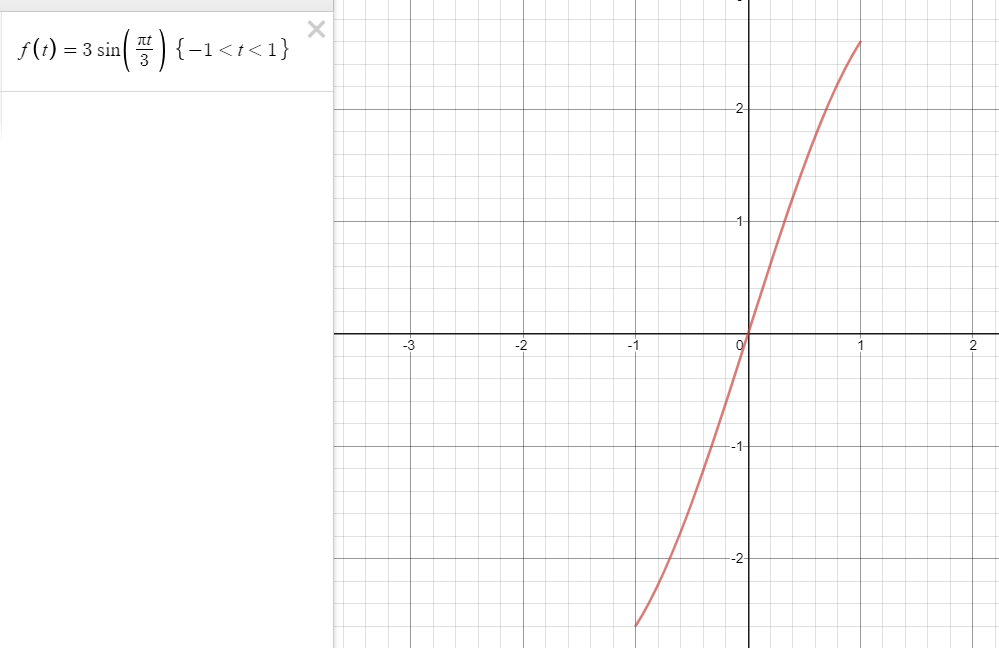
\includegraphics[width=\linewidth]{a.png}
 
    \textcolor{hwColor}{
      $f(t)=\dfrac{a_0}{2}+\sum\limits_{r=1}^{\infty}\left[a_r cos(\dfrac{2\pi r}{L}t)+b_r sin(\dfrac{2\pi r}{L}t)\right]$ 
    } 

    \textcolor{hwColor}{
      $a_0=\dfrac{2}{L}\bigints_{x_0}^{x_0+L}f(t)dt$ \\ 
      $a_r=\dfrac{2}{L}\bigints_{x_0}^{x_0+L}f(t) cos(\dfrac{2\pi r}{L}t)dt$ \\ 
      $b_r=\dfrac{2}{L}\bigints_{x_0}^{x_0+L}f(t) sin(\dfrac{2\pi r}{L}t)dt$ \\ 
    }

    \textcolor{hwColor}{ 
      \rule{15cm}{0.4pt}
    }

    \textcolor{hwColor}{ 
      L=2 \\ 
      $a_0=\dfrac{2}{2}\bigints_{-1}^{1}3sin(\dfrac{\pi t}{3})dt=3 \bigints_{-1}^{1}sin(\dfrac{\pi t}{3})dt$ \\
    }

    \textcolor{hwColor}{
      $a_r=\dfrac{2}{2}\bigints_{-1}^{1}3sin(\dfrac{\pi t}{3}) cos(\dfrac{2\pi rt}{2})dt=3\bigints_{-1}^{1}sin(\dfrac{\pi t}{3}) cos(\pi rt)dt$ \\ 
    } 

    \textcolor{hwColor}{
      $b_r=\dfrac{2}{2}\bigints_{-1}^{1}3sin(\dfrac{\pi t}{3}) sin(\dfrac{2\pi r}{2}t)dt=3\bigints_{-1}^{1}sin(\dfrac{\pi t}{3}) sin(\pi rt)dt$ \\ 
    }

    \textcolor{hwColor}{
      $f(t)=\dfrac{3 \bigints_{-1}^{1}sin(\dfrac{\pi t}{3})}{2}$ \\
      $+\sum\limits_{r=1}^{\infty}\left[\left(3\bigints_{-1}^{1}sin(\dfrac{\pi t}{3}) cos(\pi rt)dt\right) cos(\pi rt)+\left(3\bigints_{-1}^{1}sin(\dfrac{\pi t}{3}) sin(\pi rt)dt\right) sin(\pi rt)\right]$
    }
    

  \item Continue the previous problem:  calculate the integrals and write the fully simplified result for the Fourier series.

    \textcolor{hwColor}{
      $a_0=\dfrac{2}{2}\bigints_{-1}^{1}3sin(\dfrac{\pi t}{3})dt=3 \bigints_{-1}^{1}sin(\dfrac{\pi t}{3})dt=3\left(-\dfrac{3}{\pi}cos(\dfrac{\pi}{3}t)\right)\Big|_{-1}^{1}$ \\
      $=3\left[-\dfrac{3}{\pi}cos(\dfrac{\pi}{3})+\dfrac{3}{\pi}cos(-\dfrac{\pi}{3})\right]=3 \times 0 \Longrightarrow a_0=0$
    }

    \bigbreak

    \textcolor{hwColor}{
      $a_r=3\bigints_{-1}^{1}sin(\dfrac{\pi t}{3}) cos(\pi rt)dt=\dfrac{3}{2}\bigints_{-1}^{1}\left[sin(\dfrac{\pi +3\pi r}{3}t)+sin(\dfrac{\pi - 3\pi r}{3}t)\right]dt$ \\
      $=\dfrac{3}{2}\left[\bigints_{-1}^{1}sin(\dfrac{\pi +3\pi r}{3}t) dt+\bigints_{-1}^{1}sin(\dfrac{\pi - 3\pi r}{3}t) dt\right]$ \\
      $=\dfrac{3}{2} \left[-\dfrac{3}{\pi + 3\pi r}cos(\dfrac{\pi + 3\pi r}{3}t)\Big|_{-1}^{1}-\dfrac{3}{\pi -3\pi r}cos(\dfrac{\pi -3\pi r}{3}t)\Big|_{-1}^{1}\right]$ \\
      $\Longrightarrow a_r=0$
    }

    \bigbreak
  
    \textcolor{hwColor}{
      $b_r=3\bigints_{-1}^{1}sin(\dfrac{\pi t}{3}) sin(\pi rt)dt=-\dfrac{3}{2}\left[\bigints_{-1}^{1} cos(\dfrac{\pi + 3\pi r}{3}t)dt-\bigints_{-1}^{1}cos(\dfrac{\pi - 3\pi r}{3}t)dt\right]$ \\
      $=-\dfrac{3}{2}\left[\dfrac{3}{\pi + 3\pi r}sin(\dfrac{\pi + 3\pi r}{3}t)\Big|_{-1}^{1}+\dfrac{3}{\pi - 3\pi r}sin(\dfrac{\pi - 3\pi r}{3}t)\Big|_{-1}^{1}\right]$ \\
      $=-\dfrac{3}{2} \left[\dfrac{6}{\pi + 3\pi r}sin(\dfrac{\pi + 3\pi r}{3})+\dfrac{6}{\pi - 3\pi r}sin(\dfrac{\pi - 3\pi r}{3})\right]$ \\
      $=-\dfrac{3}{2}\left[\left(\dfrac{6}{\pi + 3\pi r}\dfrac{\sqrt{3}}{2}(-1)^r\right)+\left(\dfrac{6}{\pi - 3\pi r}\dfrac{\sqrt{3}}{2}(-1)^r\right)\right]$ \\
      $=-\dfrac{9\sqrt{3}}{2}(-1)^r\left[\dfrac{2\pi}{(\pi +3\pi r)(\pi - 3\pi r)}\right]$ \\
      \\
      $\Longrightarrow b_r=-\dfrac{9\sqrt{3}(-1)^r}{\pi - 9\pi r^2}$
    }

    \bigbreak

    \textcolor{hwColor}{
      $f(t)=\sum\limits_{r=1}^{\infty} -\dfrac{9\sqrt{3}(-1)^r}{\pi - 9\pi r^2} sin(\pi rt)$
    }
  
  \item Consider the following periodic function, defined over one period as given: 
  $$
    f(t)=t(1-t) ,\;0<t<1
  $$
  graph it (good quality hand-drawn graphs are acceptable) and set up the integrals necessary to calculate the \emph{real} Fourier series.

    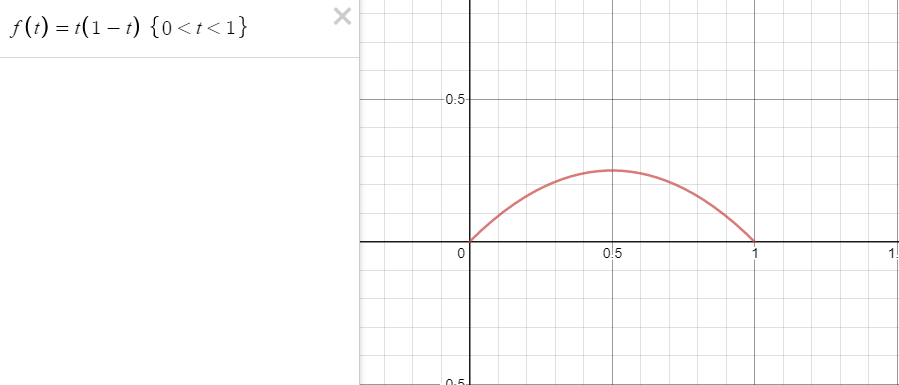
\includegraphics[width=\linewidth]{b.png}

    \textcolor{hwColor}{
      $f(t)=\dfrac{a_0}{2}+\sum\limits_{r=1}^{\infty}\left[a_r cos(\dfrac{2\pi r}{L}t)+b_r sin(\dfrac{2\pi r}{L}t)\right]$ 
    } 

    \textcolor{hwColor}{
      $a_0=\dfrac{2}{L}\bigints_{x_0}^{x_0+L}f(t)dt$ \\
      $a_r=\dfrac{2}{L}\bigints_{x_0}^{x_0+L}f(t) cos(\dfrac{2\pi r}{L}t)dt$ \\
      $b_r=\dfrac{2}{L}\bigints_{x_0}^{x_0+L}f(t) sin(\dfrac{2\pi r}{L}t)dt$ \\
    }

    \textcolor{hwColor}{ 
      \rule{15cm}{0.4pt}
    }

    \textcolor{hwColor}{ 
      L=1 \\ 
      $a_0=2\bigints_{0}^{1}t(1-t)dt$ \\
    }

    \textcolor{hwColor}{
      $a_r=2\bigints_{0}^{1}t(1-t) cos(2\pi rt)dt$ \\
    }

    \textcolor{hwColor}{
      $b_r=2\bigints_{0}^{1}t(1-t) sin(2\pi rt)dt$ \\
    }
  
  \item Continue the previous problem:  calculate the integrals and write the fully simplified result for the Fourier series. 
  
    \textcolor{hwColor}{ 
      $a_0=2\bigints_{0}^{1}t(1-t)dt=2\left[\dfrac{t^2}{2}-\dfrac{t^3}{3}\right]\Big|_{0}^{1}=\dfrac{1}{3}$ \\
    }

    \textcolor{hwColor}{
      $a_r=2\bigints_{0}^{1}t(1-t) cos(2\pi rt)dt=2\left[\dfrac{(t-t^2)sin(2\pi rt)}{2\pi r}-\bigints \dfrac{1}{2 \pi r} sin(2\pi rt)(1-2t)dt\right]$ \\
      $=2\left[\dfrac{(t-t^2)sin(2\pi rt)}{2\pi r}-\dfrac{1}{2\pi r}\left[-\dfrac{(1-2t)cos(2\pi rt)}{2\pi r}-\dfrac{sin(2\pi rt)}{2 \pi^2 r^2}\right]\right]$ \\
      $=\left(\dfrac{(t-t^2)sin(2 \pi rt)}{\pi r}+\dfrac{1}{2 \pi^2 r^2} \left[(1-2t)cos(2\pi rt)+\dfrac{sin(2 \pi rt)}{\pi r}\right]\right)\Big|_{0}^{1}$ \\
      $=\dfrac{1}{2 \pi^2 r^2}\left[(1-2)cos(2 \pi r)+\dfrac{sin(2 \pi r)}{\pi r}\right]-\dfrac{1}{2 \pi^2 r^2}$ \\
      $=\dfrac{1}{2 \pi^2 r^2}\left[\dfrac{sin(2 \pi r)}{\pi r}-cos(2 \pi r)-1\right]$ \\
      Because $r=1,2,3,...$ $sin(2 \pi r)=0$ and $cos(2 \pi r)=1$ \\
      $=\dfrac{1}{2 \pi^2 r^2}(-1-1)$ \\
      $\Longrightarrow a_r=-\dfrac{1}{\pi^2 r^2}$
    }

    \bigbreak

    \textcolor{hwColor}{
      $b_r=2\bigints_{0}^{1}t(1-t) sin(2\pi rt)dt$ \\ 
      $=2\left[-\dfrac{(t-t^2)cos(2\pi rt)}{2 \pi r}+ \bigints \dfrac{1}{2\pi r}cos(2 \pi rt)(1-2t)dt\right]$ \\
      $=2\left[-\dfrac{(t-t^2)cos(2\pi rt)}{2 \pi r}+\left(\dfrac{(1-2t)sin(2\pi rt)}{2 \pi r}-\bigints -2\dfrac{sin(2\pi rt)}{2 \pi r}dt\right)\right]$ \\
      $=2\left[-\dfrac{(t-t^2) cos(2 \pi rt)}{2 \pi r}+\dfrac{(1-2t)sin(2 \pi rt)}{2 \pi r}-\dfrac{cos(2 \pi rt)}{2 \pi^2 r^2}\right]$ \\
      $=\left[-\dfrac{(t-t^2) cos(2 \pi rt)}{\pi r}+\dfrac{(1-2t)sin(2 \pi rt)}{\pi r}-\dfrac{cos(2 \pi rt)}{\pi^2 r^2}\right]\Big|_{0}^{1}$ \\
      $=-\dfrac{sin(2\pi r)}{\pi r}-\dfrac{cos(2 \pi r)}{\pi^2 r^2}-\dfrac{1}{\pi^2 r^2}$ \\
      Because $r=1,2,3,...$ $sin(2 \pi r)=0$ and $cos(2 \pi r)=1$ \\
      $=-\dfrac{1}{\pi^2 r^2}-\dfrac{1}{\pi^2 r^2}$ \\
      \\
      $\Longrightarrow b_r=-\dfrac{2}{\pi^2 r^2}$
    }
  
  \item Consider the following periodic function, defined over one period as given: 
  $$
  f\left( t\right) =t\left( 1-t\right) ,\;-1/2<t<1/2
  $$
  graph it (good quality hand-drawn graphs are acceptable) and set up the integrals necessary to calculate the \emph{real} Fourier series. 
  
  
  \item Continue the previous problem:  calculate the integrals and write the fully simplified result for the Fourier series. 
  
  
  \item Consider the following periodic function, defined over one period as given: 
  \[
  f\left( t\right) =\cosh \left( 2t\right) ,\;0<t<1
  \]
  graph it (good quality hand-drawn graphs are acceptable) and set up the integrals necessary to calculate the \emph{complex} Fourier series. 
  
  
  \item Continue the previous problem:  calculate the integrals and write the fully simplified result for the Fourier series. 
  
  
  \item Consider the following periodic function, defined over one period as given: 
  \[
  f\left( x\right) =\left\{ 
  \begin{array}{rrr}
  \left( 1-2x\right) ^{2} & \, & 0<x<1 \\ 
  -\left( 3-2x\right) ^{2} & \, & 1<x<2
  \end{array}
  \right. 
  \]
  graph it (good quality hand-drawn graphs are acceptable) and set up the integrals necessary to calculate the \emph{complex} Fourier series. 
  
  
  \item Continue the previous problem:  calculate the integrals and write the fully simplified result for the Fourier series. 
  
  
  \end{enumerate}

\pagebreak

\textbf{Problem set on first order ordinary differential equations} (40 points)

\begin{enumerate}

  \item {\bf The water jug} 
  
  A cubic box (of side L=3 m) is initially filled with water up to a height  $h$. The water flows out of the box through a circular hole cut in the bottom. The diameter of the hole is $d=0.1$ m. 
  
  \begin{enumerate}
  
    \item Derive a differential equation for $h=h(t)$ where $t$ is time. [Hint: you will need to use the Torricelli's law which expresses the velocity of the water flowing through the hole for a given height  $h$:  $v=\sqrt{2 g h}$. Here $g$ is the acceleration due to gravity.  ]
    
    \item solve the differential equation using $h(0)=2$ m as initial condition. 
    
    \item find how much time elapses until the box is completely empty, for $h(0)=2$ m. 
    
    \item graph (hand-drawing acceptable) the function $h(t)$. 
  
  \end{enumerate}
  
  
  \item {\bf The leaking neutrino detector} 
  
  A small neutrino detector has the shape of a  cylindrical tank. The area of the base of the cylinder is $A=0.03~{\rm m^2}$ and the height is $L=1$ m. Scientists plan to fill the tank with ultrapure water, at a rate of 3 liters per minute. Due to a human error, the detector has a leak at the bottom\footnote{Neutrino detectors occasionally do leak. If you are curious, search for the history of leaks in the SuperKamiokande detector (it took many years to find it and fix it) and in the Borexino detector. }, so there will be a loss of water. Every minute, 10\% of the total volume of water present in the tank will be lost through the leak.  
  
  \begin{enumerate}
  
    \item Derive a differential equation for the volume of water in the tank, $V=V(t)$ where $t$ is time. 
    
    \item Setting as $t=0$ the time when water starts to be poured into the tank (which is initially empty), find the time that must pass until the level of the water in the tank is $h=0.5$ m.
    
    \item Establish if the tank will ever be completely full. 
  
  \end{enumerate}
  
    
  \item {\bf Calculating the air pressure profile of a planet}
  
    Consider an idealized model of the Earth's atmosphere, which is in perfect thermodynamical equilibrium and free from atmospheric perturbations.  Call $y$ the altitude with respect to the Earth's surface, so that $y=0$ on the ground and $y>0$ above ground. Let $g$ be the acceleration of gravity, $M$ the mass of one mole of air, and $T$ the temperature. Assume that the  equation of state of a perfect gas ($PV=nRT$) is valid for atmospheric air. 
  
    Write a differential equation for the atmospheric pressure as a function of the altitude, $P=P(y)$, and solve it, for two different cases:
  
    \begin{enumerate}
  
    \item $T$ is a constant (does not depend on $y$).
  
    \item $T$ decreases linearly with altitude: $T(y)=T_0(1-\alpha y)$ ($\alpha>0$)
      
      \end{enumerate}
      
    {\it [Hints: consider an infinitesimal volume of air, and reason about balancing the forces due to pressure and weight. Explain your reasoning carefully. Use the equation of state of a perfect gas to express the mass density of air.  ]}
  
  
  \item {\bf Nuclear decay chain}
  
  
  Consider an sample of atomic nuclei, of species $X_1$. This species is unstable, and the number of nuclei that decay per unit time is proportional to the number of nuclei in the sample, $N_1$. Let the constant of proportionality be $k_1$.     
  
    \begin{enumerate}
  
    \item  write a differential equation for $N_1(t)$ and solve it, for $N_1(0)=N_0$.  In doing so, assume that $k_1>0$ and be careful in setting the signs. 
  
    \item Let us now consider the daughter nucleus, $X_2$, which is produced in the decay of $X_1$. $X_2$ is unstable: let $N_2$ and $k_2$ be its abundance (time-dependent) and decay constant.  Write a differential equation for $N_2(t)$ and solve it for the case where $N_2(0)=0$ and $N_1(0)=N_0$.
  
      \item With reference to your result for $N_2(t)$, is $N_2(t)\geq 0$ in all cases, or some extra condition on the decay constants is required to ensure that?  Comment as adequate.   
      
      \end{enumerate}
  
  \end{enumerate}

  \pagebreak

  \textbf{Exercises set on first order ordinary differential equations} (5 points)

  \begin{enumerate}


    \item Find the general solutions to the following inhomogeneous first-order linear differential equations by using the integrating factor method. 
    
    \begin{enumerate}
      \item $y^{\prime}+3y=e^{2x}$
      
      \item $y^{\prime}+3y=e^{3x}$
      
      \item $y^{\prime}+3y=e^{-3x}$
      
      \item $y^{\prime}+3y=4$
      
      \item $y^{\prime}-y=2x^{2}$
      
      \item $y^{\prime}-y=\cos x$
      
      \item $y^{\prime}+y=\sinh x$
      
      \item $y^{\prime}+y=xe^{2x}$
    \end{enumerate}
    
    \item Some of the following differential equations are exact; others are not.Solve those that are, and attempt to solve those that are not by finding an appropriate integrating factor.
    
    \begin{enumerate}
      \item $(3x^{2}+y^{2})\,dx+2xy\,dy=0$.
      
      \item $\left( ye^{x}-\sin x\right) \,dx-\left( y^{2}-e^{x}\right) \,dy=0$.
      
      \item $y\left( 1+xy\right) \,dx+\left( 2y-x\right) \,dy=0$.
      
      \item $\left( e^{x}+y/x\right) \,dx+\left( \ln x+1/y\right) \,dy=0,$ $x>0$.
      
      \item $\left( x^{2}-y^{2}\right) \,dy-2xy\,dx=0.$
    \end{enumerate}
    
    
    \item  For each of the following equations, show that the equation is either homogeneous or isobaric (i.e., scale invariant). Find the general solution (you can leave the final antiderivative undone if it is particularly complicated, but please simplify and reduce fully up to that final step.). 
    
    \begin{enumerate}
      \item $xy^{\prime }+y^{2}/x=xe^{y/x}$
      
      \item $\left( x^{2}+y^{2}\right) \,dy+\left( y^{2}-x^{2}\right) \,dx=0$
      
      \item $\left( x+y^{2}\right) \,dy+y\,dx=0$
      
      \item $\left( y+x^{2}\right) \,dy-x^{3}\,dx=xy \sin \left( x^{2}/y\right) \, dx$
    \end{enumerate}
  \end{enumerate}

  \pagebreak

\end{document}
